\documentclass[11pt]{article} % For LaTeX2e
\usepackage{rldm2019, palatino}
\usepackage{graphicx}
\usepackage{amsfonts, amsmath}
\usepackage{algorithm, algpseudocode}%
\usepackage[numbers,super]{natbib}

\title{Anxiety, avoidance, and sequential evaluation}

\author{
Samuel Zorowitz \\
Princeton Neuroscience Institute\\
Princeton University\\
Princeton, NJ 08540 \\
\texttt{zorowitz@princeton.edu} \\
\And
Ida Momennejad \\
Columbia University\\
New York, NY 10027 \\
\texttt{ida.m@columbia.edu} \\
\And
Nathaniel D. Daw \\
Princeton Neuroscience Institute\\
and Department of Psychology\\
Princeton University\\
Princeton, NJ 08540 \\
\texttt{ndaw@princeton.edu} \\
}

\newcommand{\fix}{\marginpar{FIX}}
\newcommand{\new}{\marginpar{NEW}}

\begin{document}

\maketitle

\begin{abstract}
Anxiety disorders are characterized by a range of aberrations in the processing and response to threat, but there is little clarity what core pathogenesis might underlie these symptoms. Here we propose a decision theoretic analysis of maladaptive avoidance and embody it in a reinforcement learning model, which shows how a localized bias in beliefs can formally explain a range of phenomena related to anxiety. The core observation, implicit in standard decision theoretic accounts of sequential evaluation, is that avoidance should be protective: if danger can be avoided later, it poses no threat now. We show how a violation of this assumption --- a pessimistic, false belief that later avoidance will be unsuccessful --- leads to a characteristic propagation of fear and avoidance to situations far antecedent of threat. This single deviation can explain a surprising range of features of anxious behavior, including exaggerated threat appraisals, fear generalization, and persistent avoidance. Simulations of the model reproduce laboratory demonstrations of abnormal decision making in anxiety, including in situations of approach-avoid conflict and planning to avoid losses. The model also ties together a number of other seemingly disjoint issues in anxious disorders. For instance, learning under the pessimistic bias captures a hypothesis about the role of anxiety in the later development of depression. The bias itself offers a new formalization of classic insights from the psychiatric literature about the central role of maladaptive beliefs about control and self-efficacy in anxiety. This perspective is importantly different from previous computational accounts of beliefs about control in mood disorders, which neglected the sequential aspects of choice.
\end{abstract}

\keywords{
anxiety; avoidance; fear generalization; decision theory; computational psychiatry
}

\acknowledgements{This research was supported in part by NIH grant MH10917, part of the CRCNS program.} 

\startmain

\section{Introduction}

Anxiety disorders are characterized by aberrations in the processing of and response to threat \citep{dsm5, ClarkBeck2011}. Specifically, anxiety is associated with exaggerated threat appraisal, or the tendency to perceive threat as disproportionately greater in likelihood and severity than is warranted; fear generalization, or the spread of fear to situations distantly associated with the primary threat \citep{dymond2015}; and persistent avoidance behavior, which can be disruptive to everyday function \citep{Arnaudova2017}. Though laboratory studies of learning in anxious populations have corroborated these clinical observations \citep{Harle2017, norbury2018, Aylward2019}, none offer an explanation as to the root of these symptoms.

The puzzle of these symptoms is particularly sharp from a decision theoretic perspective \citep{huys2015}. Here we isolate and address a  decision theoretic paradox that, we argue, clarifies the core psychopathology: The generalization of fear and avoidance to situations far antecedent of threat violates the basic logic of evaluation over sequential trajectories of action. This is because avoidance is by nature protective: the ability to avoid in future means I need not also do so now. For instance, cars endanger pedestrians but can be reliably avoided by following traffic signals; given that, staying indoors offers no additional protection from accidents. This is an instance of a general property of evaluating actions in sequential tasks: such evaluation turns fundamentally on assumptions about subsequent events, including the agent's own subsequent choices. Typically, it is appropriate to assume that the agent will also make good choices down the line. 

This line of reasoning hints that a fundamental deficit in anxiety disorders may relate to this assumption, which otherwise should preclude the spread of avoidance. Indeed, anxiety disorders are associated with pessimistic beliefs about the future \citep{ClarkBeck2011}. Anxious individuals are more likely to endorse beliefs like that they are likely to encounter danger in the future and, notably, that they will be unable to mitigate it when they do. We develop this idea into a model of evaluation under pessimistic assumptions about future choices. We show that this single, localized deviation can explain a surprising range of features of anxious behavior including exaggerated threat appraisal, fear generalization, and persistent avoidance. This model also offers a new formalization of classic insights from the psychiatric literature about the central role of beliefs about control and self-efficacy in anxiety. Our perspective is importantly different from previous computational accounts of beliefs about control in mood disorders (e.g. \cite{HuysDayan2009}), which neglected the sequential aspects of choice. 

\section{Model description}

We model anxious decision making in the context of Markov decision processes (MDPs). A standard normative assumption is that agents attempt to optimize the expected cumulative discounted reward
\begin{equation*}
Q^\pi(s,a) = r(s,a) + \gamma \sum_{s'} p(s' \mid s,a) \sum_{a'} \pi(a' \mid s') Q^\pi(s',a'),
\end{equation*}
but for any particular state-action $a$, this is necessarily defined only relative to a policy $\pi(a' \mid s')$ specifying the assumed distribution of \emph{future} choices. The return can be optimized self-consistently assuming the agent makes the return-maximizing choice at each step in the future, leading to the familiar expression for the optimal values
\begin{equation}\label{eq:bellman}
 Q^*(s,a) = r(s,a) + \gamma \sum_{s'} p(s' \mid s,a) \max_{a'} Q^*(s',a').
\end{equation}
The ``max'' operator in Eq.~\ref{eq:bellman} yields a fundamental asymmetry between approach and avoidance, as illustrated in Fig.~1. The assumption that the agent makes the return-optimizing choice at each step implies that opportunities propagate recursively to earlier steps, but avoidable dangers do not. This principle is highlighted in a toy MDP: a deterministic open gridworld with terminal states containing a single reward and punishment (Fig.~1a). The optimal state values $V^* = \max_a Q^*(s,a)$ (Fig.~1b) reflect a ``mountain'' of opportunity propagating recursively from the reward. Conversely, because harm is avoidable in this environment, its negative value is contained: all states (even those adjacent to threat) represent the opportunity for reward.

Consider an agent who instead has pessimistic expectations about events at future steps. Such returns can be adaptive to ensure robustness such as under adversarial scenarios \cite{Garcia2015}; here we propose unrealistically pessimistic assumptions as a root cause of many anxious symptoms. Although such pessimism can be encoded either in $P(s' \mid s,a)$ or $\pi(a \mid s)$, here for concreteness we adopt the $\beta$-pessimistic value function from \cite{Gaskett2003}, to define
\begin{equation*}
Q^w(s,a) = r(s,a) + \gamma \sum_{s'} p(s' \mid s,a) \left( w \max_{a'} Q^w(s',a') + (1 - w) \min_{a'} Q^w(s',a') \right)
\end{equation*}
Here, the parameter $w$ controls the degree of pessimism. An optimistic agent ($w = 1$) expects in the future to act fully in accordance with its preferences whereas a pessimistic agent ($w = 0$) expects to act contrary to its preferences. Fig.~1c,d illustrates the the consequences of different levels of pessimism for valuation in the example gridworld; here, the expectation that the agent may fail to avoid in future causes the value of threat to permeate the state space.

\begin{figure}
  \centerline{%
    \resizebox{1.0\textwidth}{!}{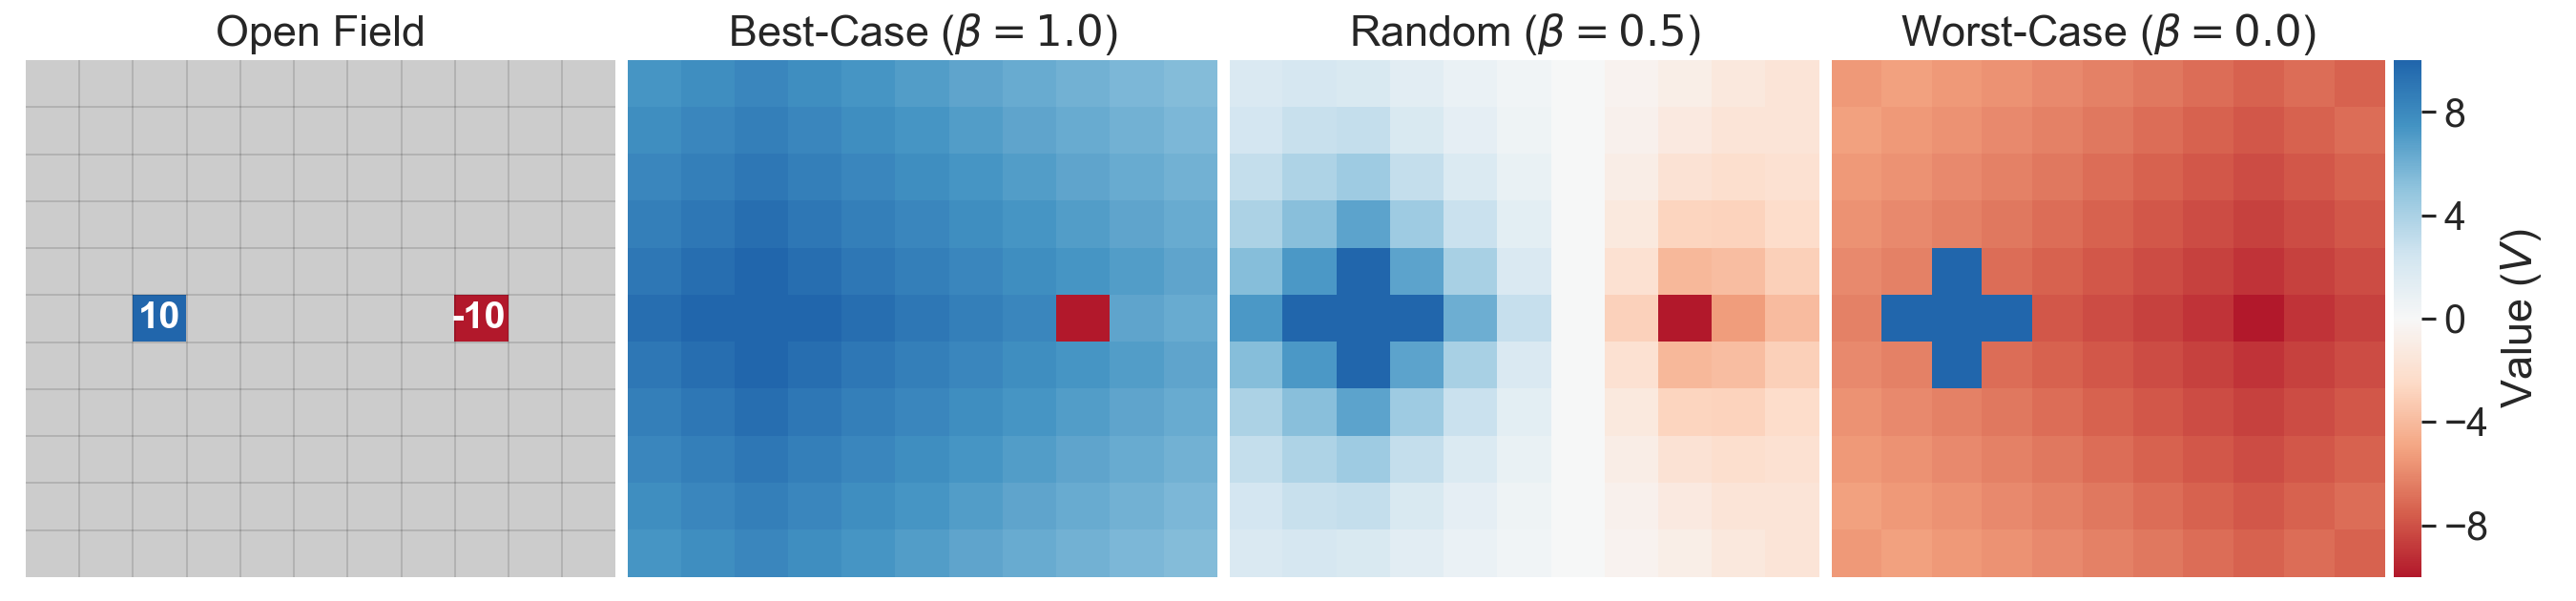
\includegraphics[trim={0 0 0 0},clip]{../../figures/01_field.png}}%
  }
  \par \textbf{Figure 1:} (A) A simple deterministic gridworld with two terminal states: one rewarding (blue) and aversive (red) state. (B) For an optimistic agent ($w=1$), all states (other than the harmful state) take on positive value. (C) For a pessimistic agent ($w=0.5$), negative value spreads from the source to antecedent states. (D) With increasing pessimism ($w=0$), the extent of the spread grows worse. (Parameters: $\gamma = 0.95$)
\end{figure}

This simple simulation --- reflecting a localized violation of a core decision theoretic assumption --- already echoes several core symptoms of anxiety disorders. The pessimistic agents in Fig~1c,d exhibit exaggerated threat appraisals (otherwise neutral states signal danger); generalization of fear (threat value spreads across the gridworld); and persistent avoidance (the agent chooses paths which maintain increasing distance from threat).

\section{Simulations}
\textbf{Approach-avoidance conflict:} One behavioral finding characteristic of anxiety disorders is unbalanced processing of approach-avoidance conflict \citep{aupperle2010}. Many of the disruptions anxiety causes to everyday functioning (e.g. avoiding social obligations for fear of possible social humiliation) can be understood in these terms. An analogous phenomenon can be measured in the laboratory. For instance, in the balloon analog risk task (BART) \citep{Lejuez2002}, participants can win money by pumping virtual balloons. With each pump, the balloon inflates and money is earned, but so too does the chance that the balloon pops (and money is lost). At any point, a participant may cash out, banking the money earned and ending the trial. Anxiety is correlated with fewer pumps and earlier cash-outs in the BART \citep{Maner2007, ramirez2015}.

As shown in Fig.~2, our model easily accommodates this result. Whereas optimistic agents pump until the marginal gain of a pump no longer offsets the chance of the balloon bursting, optimal choice under increasingly pessimistic (i.e., anxious) assumptions cashes out progressively earlier. This is because it anticipates and avoids future errors in choice resulting in the balloon popping. Our model can analogously explain other manifestations of biased approach-avoid conflict in anxiety\cite{bach2015,Mobbs2019}. One unique prediction of the model is that this bias should arise only when beliefs about \emph{future} avoidance are involved, rather than direct conflict between immediate impulses. Recent data \cite{Mobbs2019} using a predator avoidance task analogous to the BART, support this view: sub-clinical anxiety predicted earlier escape (analogous to cash-out in the BART) for slow predators (for whom future decisions to escape were a relevant consideration) but not fast ones (who would attack immediately, negating consideration of future steps).

\textbf{Aversive pruning:} Another empirical phenomenon associated with anxiety is ``aversive pruning'' in planning \cite{Huys2012, Lally2017}. This refers to the idea that when evaluating future trajectories in a sequential task like chess, people must selectively consider certain paths and neglect others. One proposal for how people accomplish this is aversive pruning \citep{Huys2012}: choice sequences involving large losses are discarded from further evaluation. For instance, although the optimal choice in the decision tree from Fig.~3a is to weather an initial large loss in order to reap the large gain that follows, people tend to disfavor this path suggesting they neglect the later gain. The degree of such pruning correlates with depressive \cite{Huys2012} and anxiety \cite{Lally2017} symptoms. Our model predicts this result (Fig.~3b), though for a somewhat different reason: in our model, pessimistic (anxious) agents neglect large gains deeper in the tree, not because they fail to consider them, but because with increasing anxiety they increasingly predict the possibility of choosing incorrectly afterward, and failing to recoup the loss. Future research could use slight variants in the decision trees to tease apart these different interpretations.

\begin{figure}
  \centerline{%
    \resizebox{1.0\textwidth}{!}{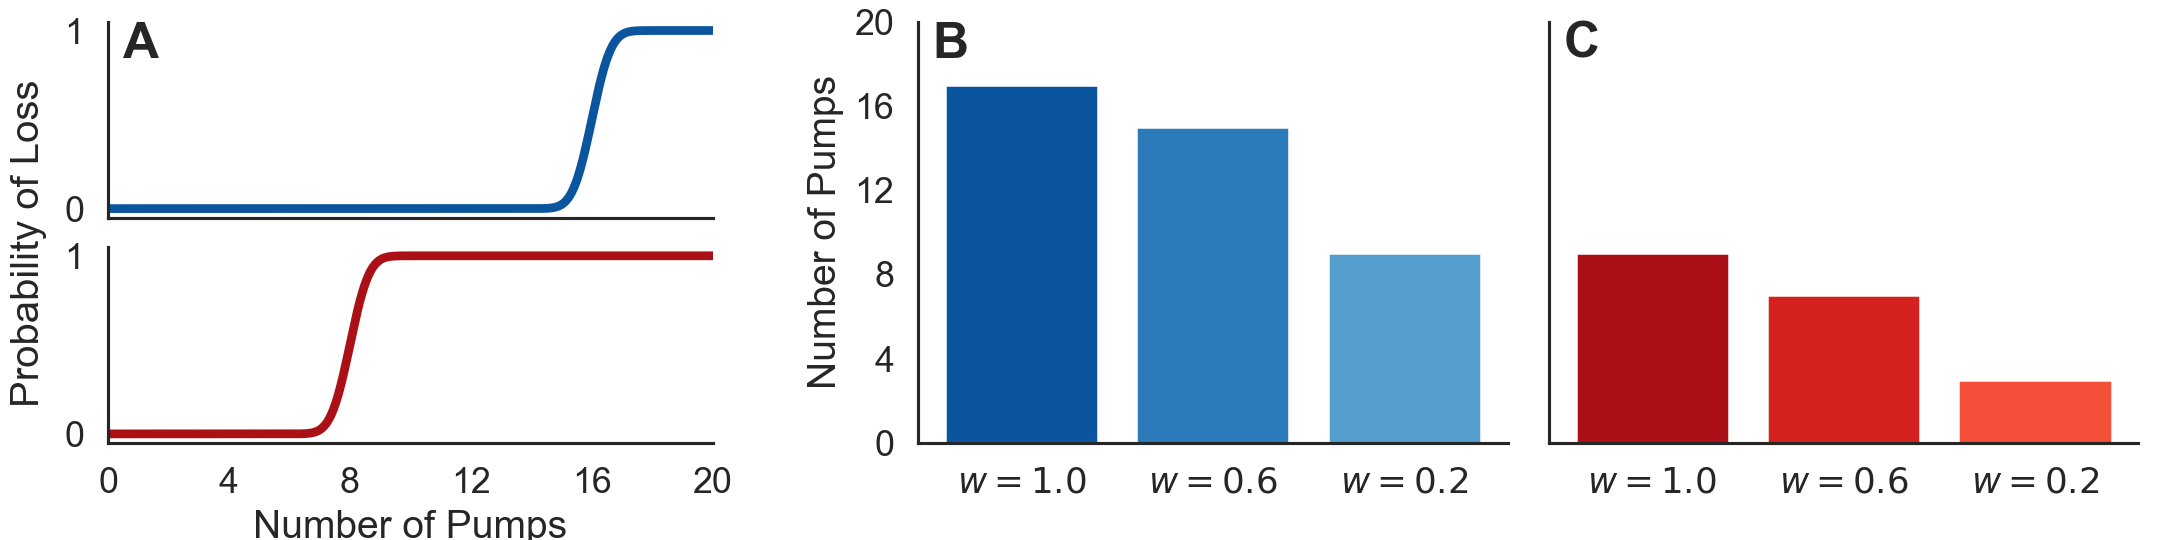
\includegraphics[trim={0 0 0 0},clip]{../../figures/02_bart.png}}%
  }
  \par \textbf{Figure 2:} (A) The Balloon Analog Risk Task (BART). The risk of balloon burst (point loss) increases with each pump. The optimal policy (number of pumps) under increasingly pessimistic valuation is presented for low (B) and high risk (C) balloons. The optimistic agent ($w=1$) prefers a policy reflecting the true environmental risk. The moderate ($w=0.6$) and strongly ($w=0.2$) pessimistic agents cash-out earlier, as is observed in anxious individuals. (Parameters: $\gamma = 1.0$)
\end{figure}

\textbf{The anxiety-depression transition:} So far, we have considered the asymptotic preferences implied the pessimistic value function. But we can also consider learning under this value function (e.g., by Q-learning or DYNA using the $\beta$-pessimistic return), the dynamics of which may speak to the progression of symptoms. 

Of note in this respect, anxiety and depression are highly comorbid, with roughly 45\% of individuals with a lifetime depression diagnosis also diagnosed with an anxiety disorder \citep{kessler2015}. One interesting proposal is that this association often arises longitudinally: in particular, that anxiety precedes certain types of depression \citep{alloy1990, jacobson2014}. The idea, in brief, is that anxiety begets avoidance and foregone reward, leading ultimately to a belief that reward is unattainable and subsequently depression. This story is borne out by simulations of learning in our model (not shown, for space) in environments like that of Fig.~1: the penumbra of negative value under pessimistic assumptions spreads gradually throughout the environment with the progress of learning, ultimately leading the agent to expect no reward and, echoing anergic symptoms of depression, forego action altogether.

A second point about learning in this model is that, because the pessimistic return ultimately spreads biased value estimates to states and actions far distant from the primary danger (e.g., Fig.~1d), it would accordingly also take a great many steps of iterative learning to correct all these misattributions, even given direct experience that the danger itself has passed. This may offer at least a partial answer to a classic puzzle in pathological avoidance, i.e. why it is so resistant to extinction \cite{moutoussis2018}.

\begin{figure}[!b]
  \centerline{%
    \resizebox{1.0\textwidth}{!}{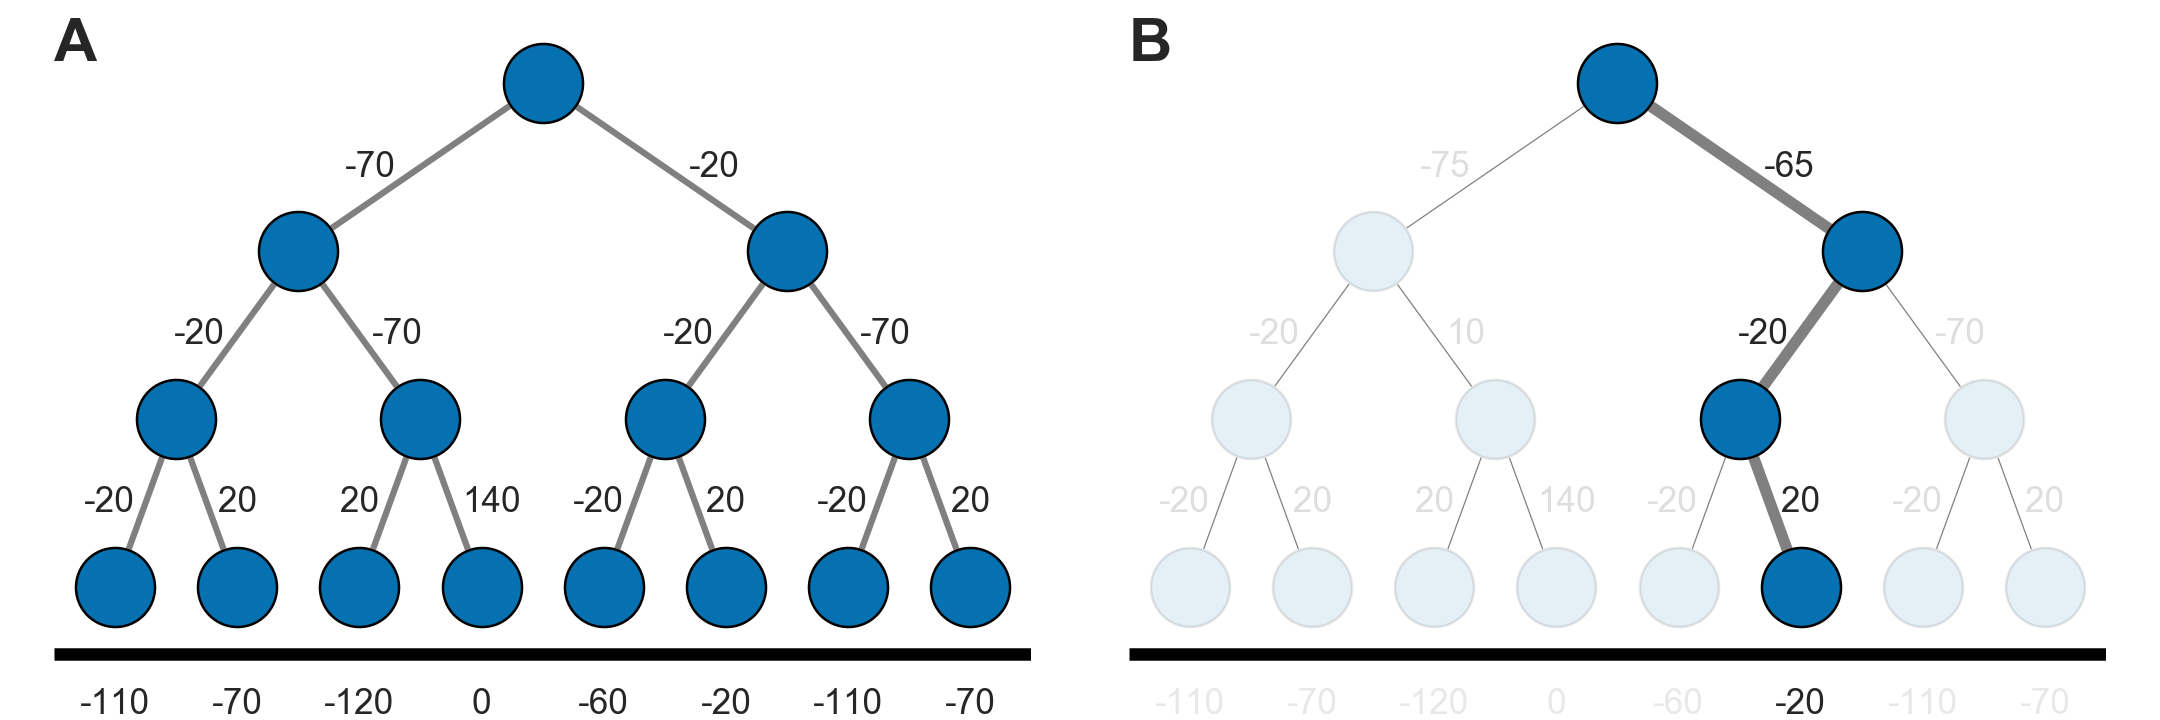
\includegraphics[trim={0 0 0 0},clip]{../../figures/04_tree_rldm.png}}%
  }
  \par \textbf{Figure 3:} (A) The decision tree environment from \cite{Huys2012} and \cite{Lally2017}. An optimistic agent ($w=1$) prefers the optimal loss-minimizing policy through the initial large loss (left branch). (B) A pessimistic agent ($w=0.5$) comes to prefer the branch without the large loss so as to avoid being unable to recoup the large initial loss. One-step rewards are presented in each state; the net value $Q$ on each path is shown numerically. (Parameters: $\gamma = 1.0$)
\end{figure}

\section{Discussion}

Central to anxiety disorders are symptoms including pessimistic inference, threat generalization, and excessive avoidance. We have presented a simple computational account suggesting how a single underlying misbelief can give rise to a range of these aberrations in learning and choice. Specifically, we showed how a failure to believe in the reliability of future self-action can effectively backpropagate negative value across states of the environment. This process results in a range of inferences and behaviors resembling those observed in clinical anxiety. Though this is by no means a complete account of anxiety, it ties together a surprisingly wide range of its symptoms.

One important ambiguity is that we have formalized pessimistic assumptions in terms of beliefs about the agent's own future actions: expecting failure, for instance, to avoid in future. Since Eq.~1 is also computed in expectation over the anticipated future environmental dynamics $p(s' \mid s,a)$, pessimism can alternatively be encoded in this distribution (e.g., a belief that the world's response to one's choices is unpredictable or adversarial). Because the Bellman equation averages out both distributions,  and because an unpredictable environment also reduces the efficacy of avoidance, either formulation can produce ultimately similar results. However from the perspective of cognitive theories of anxiety, these represent quite different maladaptive beliefs, which may be relevant, for instance, in guiding treatment.

Indeed, our account formalizes a longstanding strand of theory on the role of control in anxiety. Central to many prominent cognitive theories of anxiety in the psychiatric literature is a perceived lack of control. For example, learned helplessness theory claims that pathological anxiety results from a belief that the environment is uncontrollable, such that threat cannot be effectively mitigated \cite{alloy1990}. In contrast, Bandura's self-efficacy theory of anxiety posited that a lack of confidence in one's own ability to effectively handle threat was instead central \cite{bandura1977}. As we note above, the present model (though stated here in terms echoing Bandura's) can accommodate either variant, and they are by no means mutually exclusive. 

Finally, we are not the first to propose a formal theory of control in psychiatry using MDPs. Huys\cite{HuysDayan2009} provided a computational account of learned helplessness through simple models of one-step action-outcome contingencies. Our accounts differ particularly in our exclusive focus on control in the sequential setting, which Huys did not address. Indeed, we propose that ultimately key to anxiety is precisely the way in which evaluation in sequential tasks is necessarily reliant on expectations about future events.

\bibliographystyle{naturemag}
\small{\bibliography{rldm2019}}

\end{document}
